\section{Introduction}

\noindent
The purpose of this project was to develop a DSL targeting a particular domain which was very easy to use, feature - rich, extensible and appropriately modelled domain semantics. The domain chosen for this project was that of software system testing. System testing is a broad area so the parts of system testing covered are regression testing, functional testing, performance testing and source code repository testing.

% \subsection{Organization of Report}

\subsection{Problem}
Testing is an integral part of software development. Unit Testing frameworks like JUnit, NUnit, TestNG and ScalaTest have been around for quite some time and allow software developers to conveniently and reliably test functionality in the form of Unit Tests. Proponents of "agile methodologies" highlight the importance of Test - Driven Development to ensure that the code base is well wrapped in tests and any sorts of regressions caused by code changes can be easily tracked and fixed \cite{tdd}. Test - Driven Development also prevents legacy code from being written, as comprehensive test suites are one of the best kinds of documentation code can come with.
\bigskip

\noindent
However, there is a scarcity of System Testing frameworks that allow developers to test the entire system. System testing is a broad area and the parts of system testing covered in the scope of this project are regression testing, functional testing, performance testing and source code repository testing. The availability of such a framework will allow developers to ensure that their code has the correct functionality on a unit test level as well as a system level. The diagram below shows the different kinds of system - level testing types:
\bigskip

\begin{figure}[H]
  \centering
    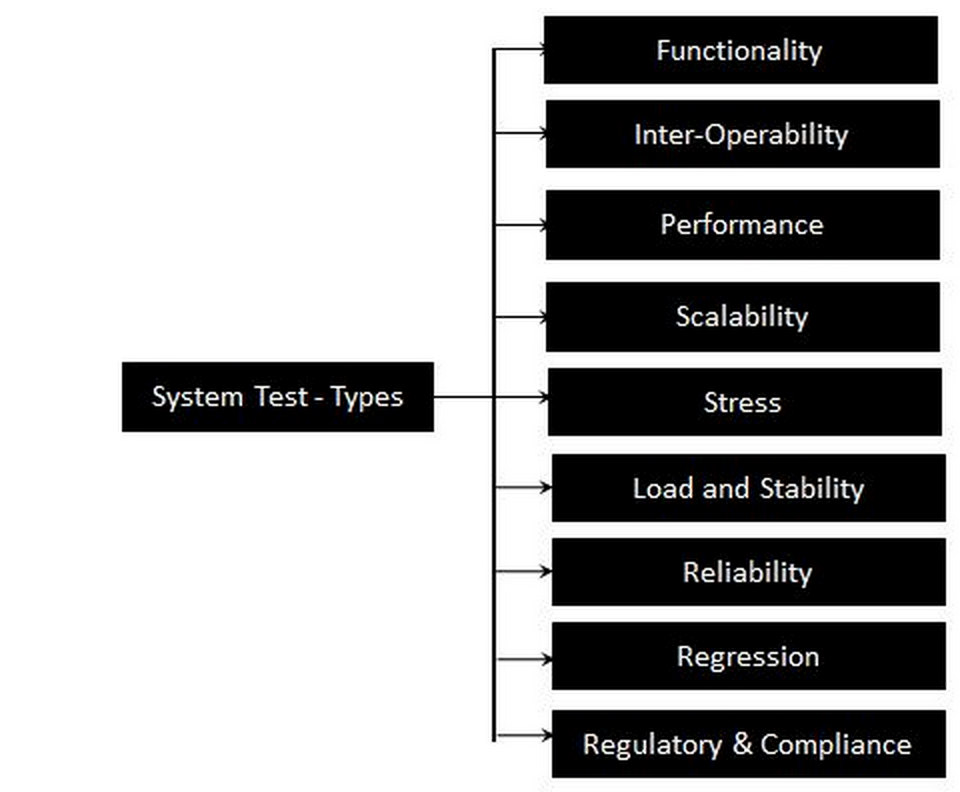
\includegraphics[height=400px]{figures/system_testing_types.png}
  \caption{Types of System Level Tests}
\end{figure}

\noindent
The DSL developed during the project provides system - level testing features such as \textbf{functional testing, regression testing, performance testing and code repository testing}. The DSL developed allows quality analysts and system testers to write test cases in a declarative, natural language like syntax and gather test statistics on tests that failed. This allows a higher level of abstraction when it comes to testing and allows them to write exhaustive test cases without concerning themselves much with code.
\newpage

\subsection{Existing Solutions and their Limitations}

\subsubsection{Selenium}
Selenium is a portable software testing framework for web applications. Selenium provides a record/playback tool for authoring tests without learning a test scripting language (Selenium IDE). It also provides a test domain-specific language (Selenese).
\bigskip

\noindent
\textbf{Limitation}: Limited to web applications that are browser based. Cannot be used for terminal based software. Selenium's selling point is that it is perfect for web browser automation

\subsubsection{JUnit}
JUnit is a popular tool for automating testing of Java classes and web-based components. JUnit can also be used with other JVM based languages like Scala. However, it is better for unit tests rather than integration tests.
\bigskip

\noindent
\textbf{Limitation}: JUnit is not built with the view of system testing or integration testing. Although integration tests are possible, they are quite cumbersome and require mocking frameworks like \textbf{Mockito} or \textbf{JMock}.
\bigskip

\subsubsection{ScalaTest} 
ScalaTest is comparable to JUnit for testing classes, traits and objects in Scala projects. The ScalaTest is highly extensible and can be extended to support custom matchers and rules.
\bigskip

\noindent
\textbf{Limitation}: ScalaTest works at source - code level and does not provide any functionality to explicitly write integration tests or system tests. 
\bigskip

\begin{figure}[ht]
\centering
\quad
\begin{minipage}[b]{0.45\linewidth}

\includegraphics[height=50px]{figures/junit_logo.png}
\caption{JUnit}
\label{fig:minipage2}
\end{minipage}
\begin{minipage}[b]{0.45\linewidth}

\includegraphics[height=50px]{figures/selenium_logo.png}
\caption{Selenium}
\label{fig:minipage2}
\end{minipage}
\end{figure}

\newpage
\subsection{Project Objectives}
The DSL developed during the course of this project had the primary objective of software system testing. System testing of software is conducted on a complete, integrated system to evaluate the system's compliance with its specified requirements.
\bigskip

\noindent
The objectives for the project were:
\begin{itemize}
\item To explore state of the art techniques in DSL development
\item To gauge the suitability of Scala for DSL development
\item To compare DSL development using a statically typed language like Scala against a dynamic language like Python
\item To develop a DSL over course of the project with certain features
\end{itemize}

\noindent
The requirements for the DSL that was developed over the course of the project were:
\begin{itemize}
\item Performance Testing
\item Functional Testing
\item Regression Testing
\item Intuitive, declarative DSL syntax for testers
\item Ease of debugging and use
\item Extensibility of the DSL
\item Ease of integration with application code
\item Closely model domain semantics
\end{itemize}

\subsection{Overview of Solution}

Over the course of this project, DSLs for software system testing were constructed. The first DSL performs \textbf{regression testing}, \textbf{performance testing} and \textbf{functional testing}. The second DSL was built for \textbf{code repository testing}. Code Repository Testing implies that a set of tests are run on individual commits/branches in the code repository and the results are summarized in a convenient, hierarchical format. This DSL was written in both Scala and Python to compare how the development was different for a dynamic language like Python in comparison to a statically typed language like Scala. The broad features of the DSLs are shown in the diagram below. For convenience, both DSLs have been collectively referred to as \textbf{Embedded DSL for System Testing}.

\begin{figure}[H]
  \centering
    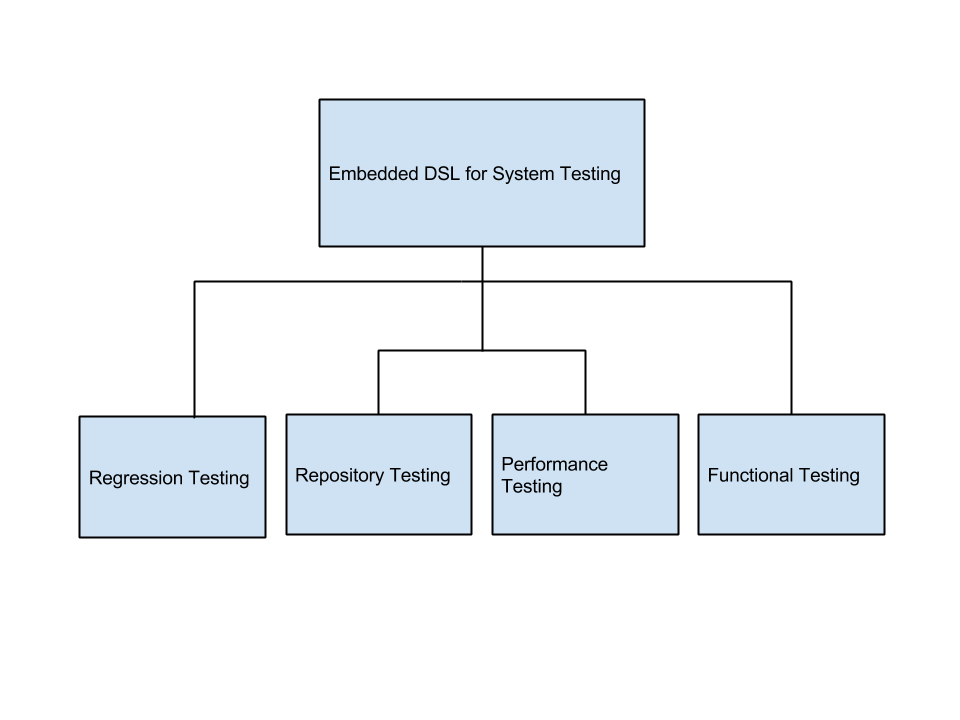
\includegraphics[width=400px]{figures/overview_of_solution.png}
  \caption{Overview of Solution}
\end{figure}

\noindent
The different testing paradigms mentioned in the diagram are explained below:
\subsubsection{Regression Testing}

\textbf{Regression Testing} is a type of software testing that seeks to uncover new software bugs, or regressions, in existing functional and non-functional areas of a system after changes such as enhancements, patches or configuration changes have been introduced \cite{Hetzel88}.
\bigskip

\subsubsection{Performance Testing}

\textbf{Performance Testing} is the process of determining the speed or effectiveness of a computer, network, software program or device{Hetzel88}. The total time taken by a particular software system to perform certain tasks is crucial for production systems. The later a performance defect is detected, the higher the cost of remediation. This is true in the case of functional testing, but more so in the case of performance testing, due to the end-to-end nature of its scope. The DSL provides a flexible way to generate \textit{timing reports} for software components and throw necessary errors in case the threshold time lapses and the process has not completed.

\subsubsection{Functional Testing}

\textbf{Functional Testing} is a quality assurance (QA) process and a type of black box testing that bases its test cases on the specifications of the software component under test \cite{Hetzel88}. The DSL developed allows functional testing of software components based on the output produced by them for certain kinds of input. These outputs can be provided as \textit{regular expressions} for flexibility.

\subsubsection{Repository Testing}

\textbf{Repository Testing} is a technique encompassing  \textbf{functional testing, regression testing and reliability testing}. A code repository (directory) has to be provided with some end to end functional tests and a \textit{time period } for testing. The DSL tests individual commits from different branches which have been made in the time period specified by the developer or tester. After testing is completed, results from all branches and relevant commits are generated and stored in a hierarchical structure for version control purposes. This version controls both the test results and branch information with the actual code enhancing \textit{maintainability} and \textit{reliability}.\bigskip

\noindent
Repository testing is also an efficient way to ensure that source code bases being worked on by several developers are in working condition and no major errors have occurred.

\newpage
\subsection{Current Applications of DSL system}

Throughout the course of the project, the DSL being developed was applied to the HIP/SLEEK verifiers being developed at NUS. The \textbf{HIP/SLEEK} systems are aimed at automatic verification of functional correctness of heap manipulating programs. HIP is a separation logic based automated verification system for a simple imperative language, able to modularly verify the specifications of heap-manipulating programs \cite{hipsleek}. 

\begin{itemize}
\item HIP Verification Functional Testing
\item SLEEK Verification Functional Testing
\item HIP/SLEEK Regression Testing
\item HIP/SLEEK Verifier Performance Testing
\item HIP/SLEEK code base Repository Testing 
\end{itemize}

\subsubsection{Migration from Legacy System to DSL}

Previously, a 2500 line Perl Script was used for functional testing. A set of shell scripts were being used for regression testing. As the System Testing DSL was being developed, the functionality of the legacy system comprising Perl and shell - scripts was being migrated over to the DSL. 

\begin{figure}[H]
  \centering
    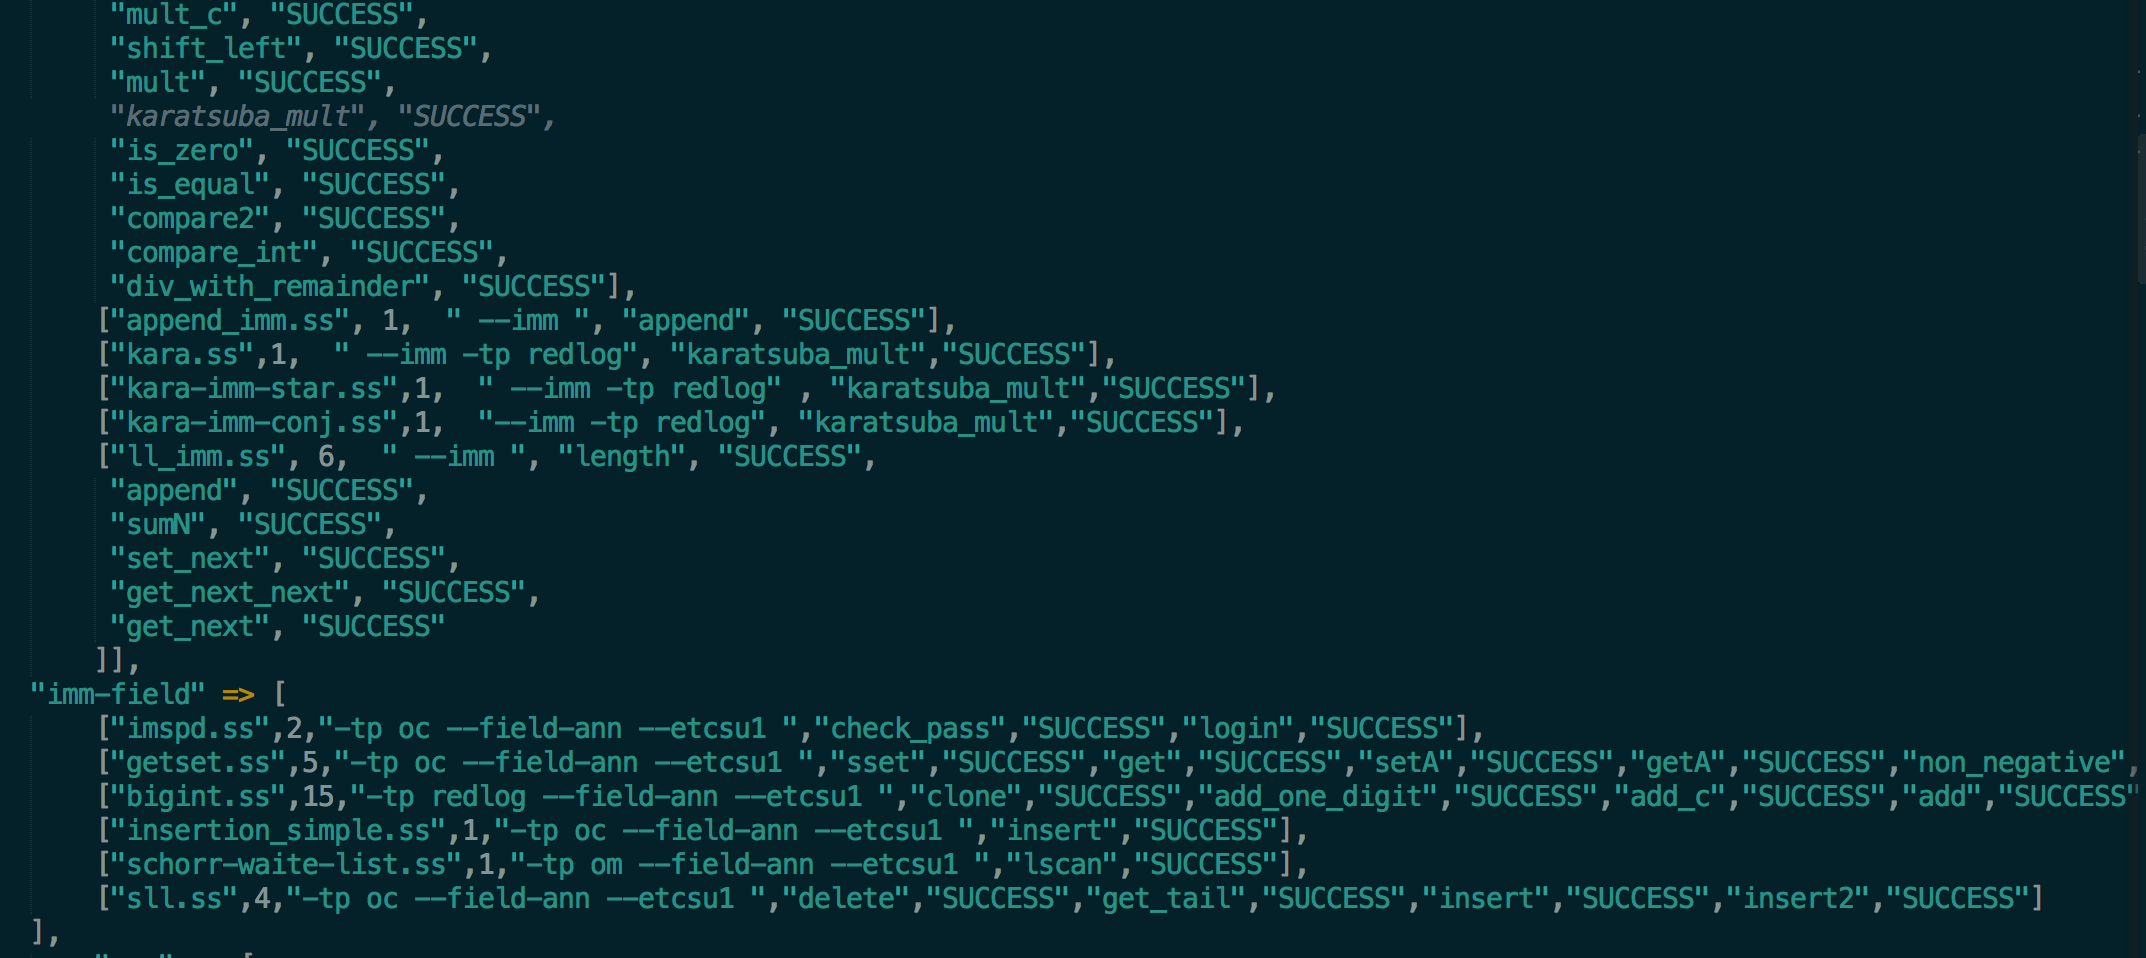
\includegraphics[width=500px]{figures/legacy1.png}
  \caption{Legacy Perl Script}
\end{figure}

\begin{figure}[H]
  \centering
    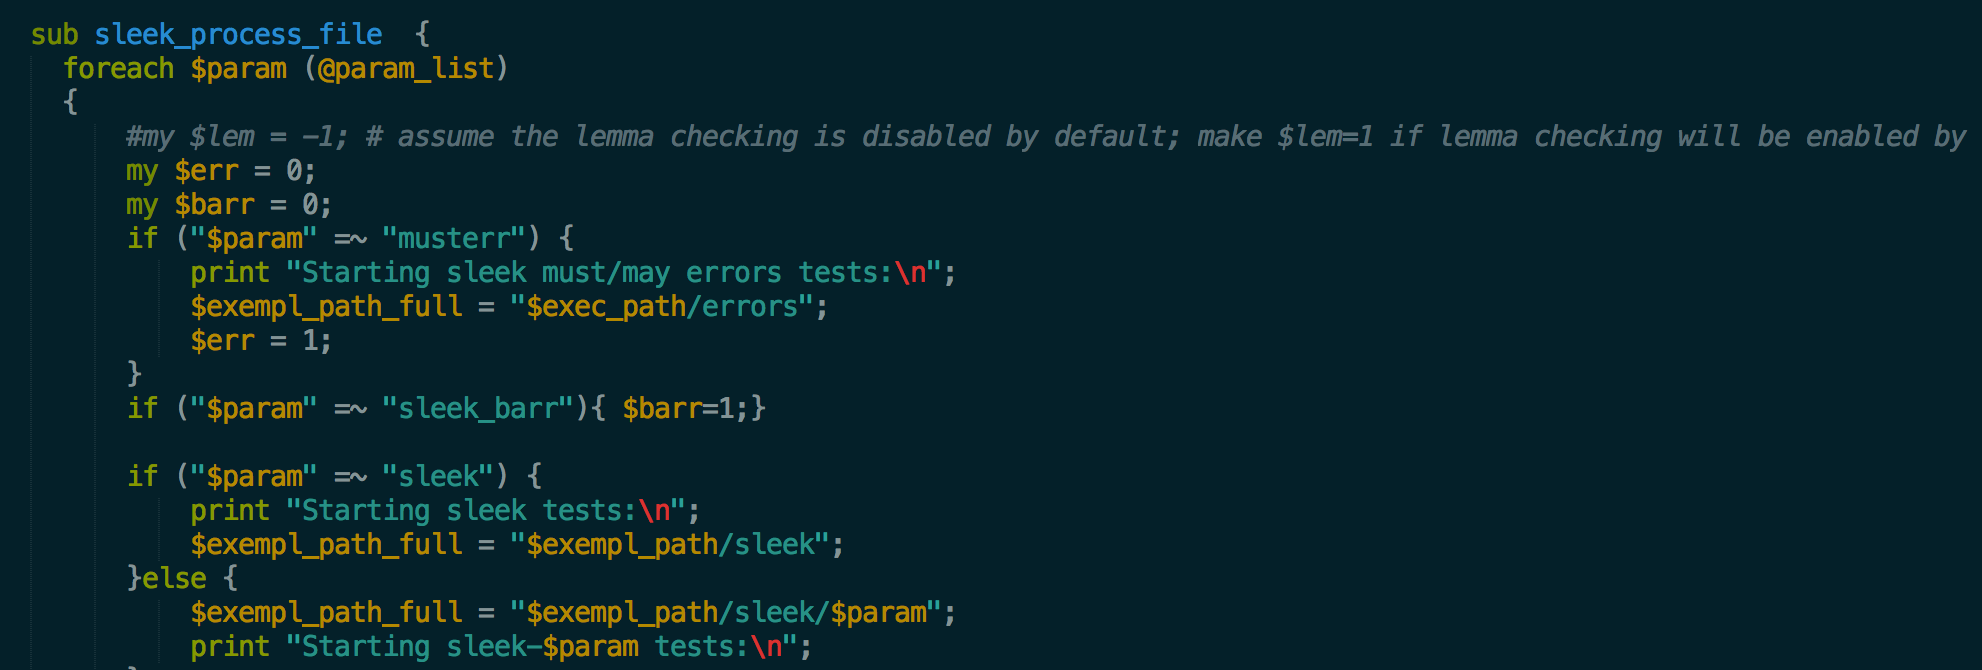
\includegraphics[width=500px]{figures/legacy2.png}
  \caption{Legacy Perl Script}
\end{figure}

\noindent
After migration, the code looks like the screen-shots below:

\begin{figure}[H]
  \centering
    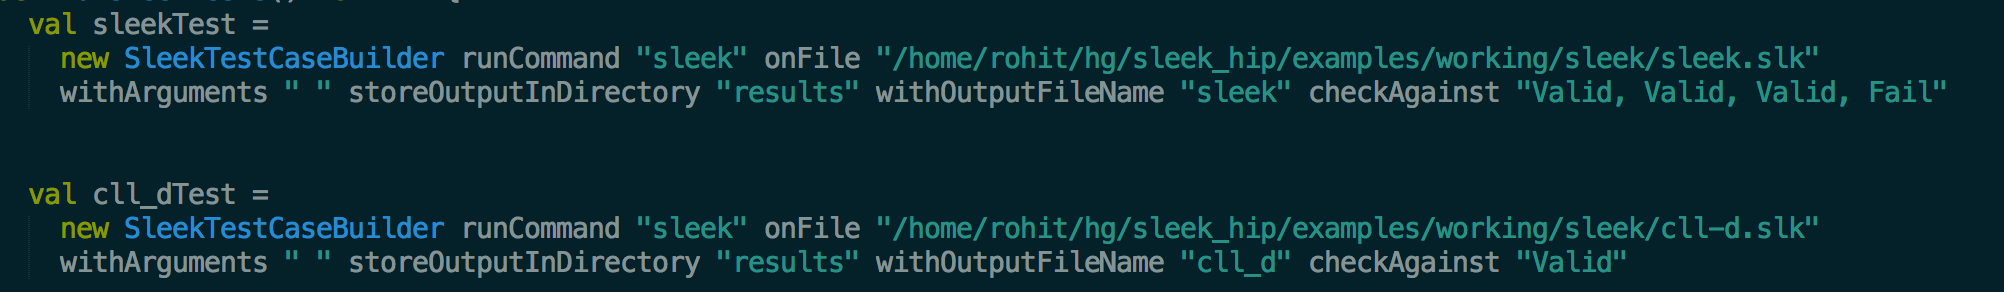
\includegraphics[width=500px]{figures/DSL_create_test.png}
  \caption{Individual Test Case Creation}
\end{figure}

\begin{figure}[H]
  \centering
    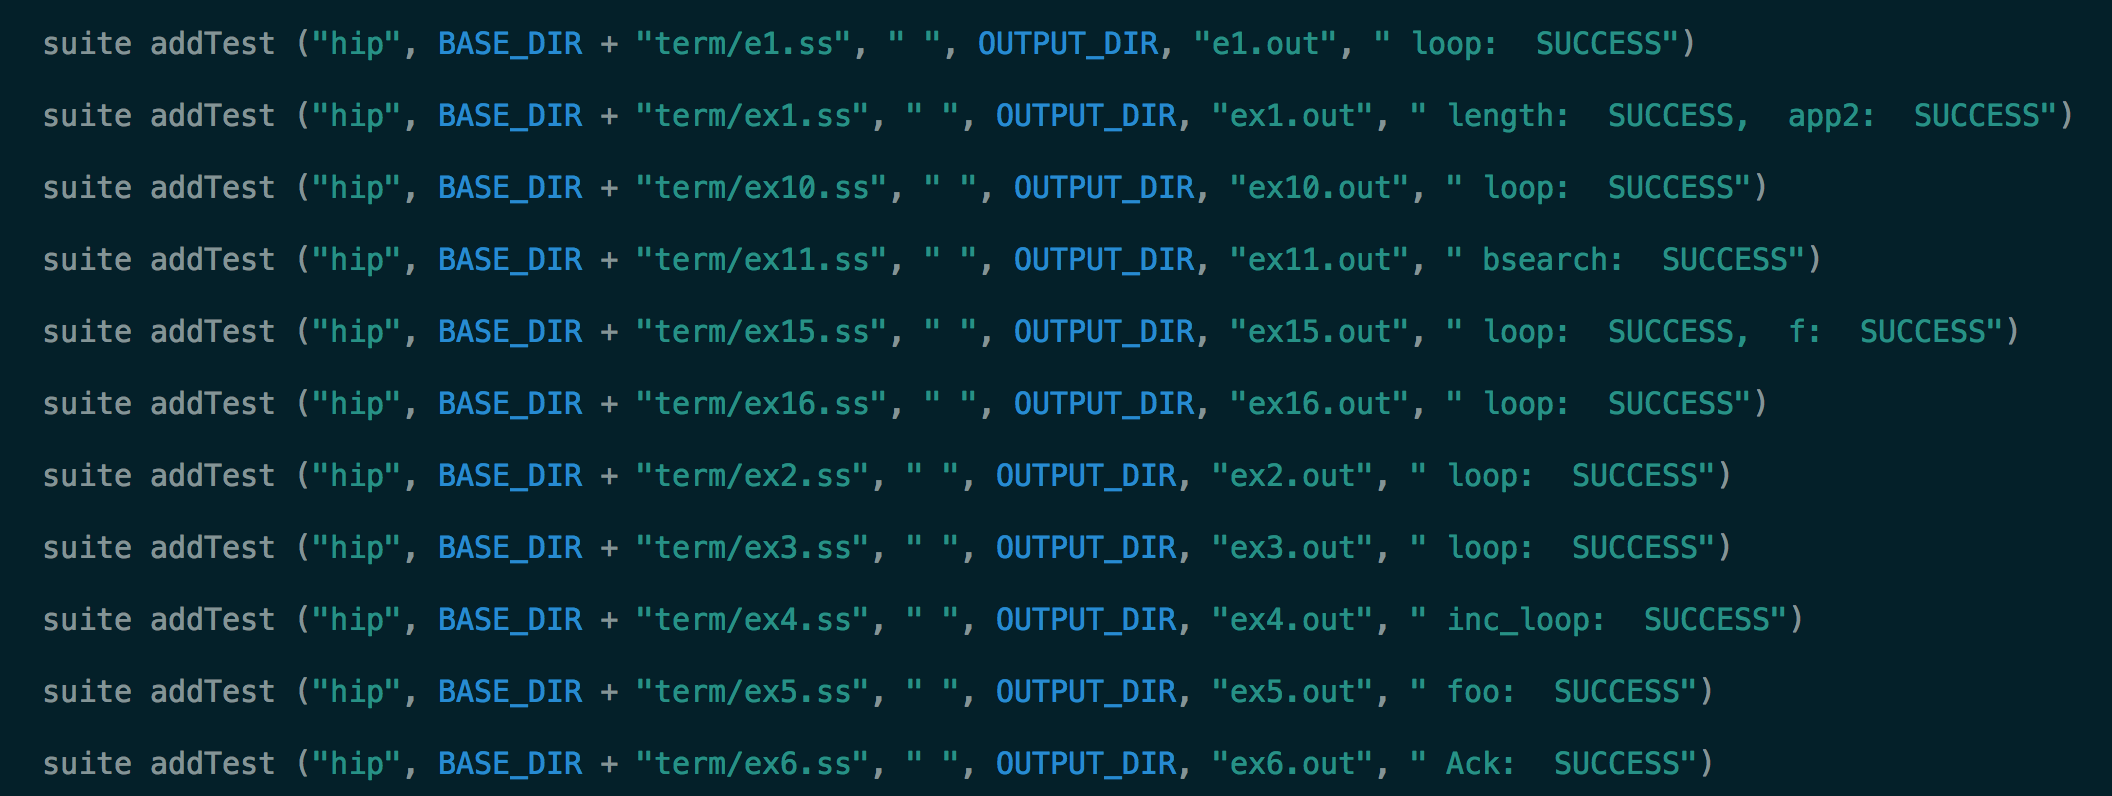
\includegraphics[width=500px]{figures/DSL_test_suite.png}
  \caption{Test Suite Creation}
\end{figure}

\subsubsection{Advantages of DSL over legacy system}
\begin{itemize}
\item Easier to maintain the test code base
\item Easier to write new tests
\item Decoupled design
\item Monolithic system instead of a collection of scripts
\item Compile time type checking leading to fewer errors
\item Extensible
\item Modular
\item The syntax of the DSL model the semantics of the domain better than general purpose languages like Perl
\item Declarative Syntax
\end{itemize}

\subsection{Key Benefits of DSL developed}
\begin{itemize}

\item \textbf{Extensibility} - The embedded DSL is well documented using ScalaDoc and types are well defined and loosely coupled. Several design patterns such as \textit{Dependency Injection, Builder, Factory and Singleton} have been applied to make the code easier to extend and maintain

\item \textbf{Highly Configurable} - Both the embedded DSL and the Reporting Tool can be easily configured using \textit{human - readable} files. Scala's \textbf{config} type has been used to configure it whereas the reporting tool in Python can be configured using a YAML file.

\item \textbf{Lightweight Library} - The DSL has been implemented as a library that 
can be easily dropped into any project by including the .JAR in the project path. Dependencies are managed using sbt (Simple Build Tool).

\item \textbf{Easy to use} - The tools are very easy to configure and use because of the library approach and decoupled design.

\item \textbf{Domain Semantics} - The DSL has types and syntax that model the domain closely and are therefore easier to read and write for domain - experts rather than general purpose languages like Java or Perl.

\item \textbf{Integration with Version Controlled Workflow} - The output generated by the system is hierarchical and can be version controlled to create a repository of results.
\end{itemize}

\subsection{Statement of Assumptions}

Some of the assumptions made during the project are:
\begin{itemize}
\item Regularity in the output produced by Systems Under Test (SUT). The output produced should be parseable using certain \textit{templates} and regular \textit{expressions}.
\item Dependencies of the system can be resolved locally
\item Functional tests are of the form: Input -\textgreater System -\textgreater Expected Output
\end{itemize}
% \subsection{Summary}
\newpage
